\documentclass[a4paper,14pt]{extreport}
\usepackage[left=1.5cm,right=1.5cm,
    top=1.5cm,bottom=2cm,bindingoffset=0cm]{geometry}
\usepackage{scrextend}
\usepackage[T1,T2A]{fontenc}
\usepackage[utf8]{inputenc}
\usepackage[english,russian,ukrainian]{babel}
\usepackage{tabularx}
\usepackage{amssymb}
\usepackage{color}
\usepackage{amsmath}
\usepackage{mathrsfs}
\usepackage{listings}
\usepackage{graphicx}
\graphicspath{ {./images/} }
\usepackage{lipsum}
\usepackage{xcolor}
\usepackage{hyperref}
\usepackage{tcolorbox}
\usepackage{tikz}
\usepackage[framemethod=TikZ]{mdframed}
\usepackage{wrapfig,boxedminipage,lipsum}
\mdfdefinestyle{MyFrame}{%
linecolor=blue,outerlinewidth=2pt,roundcorner=20pt,innertopmargin=\baselineskip,innerbottommargin=\baselineskip,innerrightmargin=20pt,innerleftmargin=20pt,backgroundcolor=gray!50!white}
 \usepackage{csvsimple}
 \usepackage{supertabular}
\usepackage{pdflscape}
\usepackage{fancyvrb}
%\usepackage{comment}
\usepackage{array,tabularx}
\usepackage{colortbl}

\usepackage{varwidth}
\tcbuselibrary{skins}
\usepackage{fancybox}
\usepackage{multirow}


\usepackage{tikz}
\usepackage[framemethod=TikZ]{mdframed}
\usepackage{xcolor}
\usetikzlibrary{calc}
\makeatletter
\newlength{\mylength}
\xdef\CircleFactor{1.1}
\setlength\mylength{\dimexpr\f@size pt}
\newsavebox{\mybox}
\newcommand*\circled[2][draw=blue]{\savebox\mybox{\vbox{\vphantom{WL1/}#1}}\setlength\mylength{\dimexpr\CircleFactor\dimexpr\ht\mybox+\dp\mybox\relax\relax}\tikzset{mystyle/.style={circle,#1,minimum height={\mylength}}}
\tikz[baseline=(char.base)]
\node[mystyle] (char) {#2};}
\makeatother

\definecolor{ggreen}{rgb}{0.4,1,0}
\definecolor{rred}{rgb}{1,0.1,0.1}
\definecolor{amber}{rgb}{1.0, 0.75, 0.0}
\definecolor{babyblue}{rgb}{0.54, 0.81, 0.94}
\definecolor{amethyst}{rgb}{0.6, 0.4, 0.8}

\usepackage{float}
\usepackage{wrapfig}
\usepackage{framed}
%for nice Code{
\lstdefinestyle{customc}{
  belowcaptionskip=1\baselineskip,
  breaklines=true,
  frame=L,
  xleftmargin=\parindent,
  language=C,
  showstringspaces=false,
  basicstyle=\small\ttfamily,
  keywordstyle=\bfseries\color{green!40!black},
  commentstyle=\itshape\color{purple!40!black},
  identifierstyle=\color{blue},
  stringstyle=\color{orange},
}
\lstset{escapechar=@,style=customc}
%}


\begin{document}
\pagecolor{white}

%----------------------------------------1
\newtcbox{\xmybox}[1][red]{on line, arc=7pt,colback=#1!10!white,colframe=#1!50!black, before upper={\rule[-3pt]{0pt}{10pt}},boxrule=1pt, boxsep=0pt,left=6pt,right=6pt,top=2pt,bottom=2pt}

\begin{titlepage}
  \begin{center}
    \large
    Національний технічний університет України \\ "Київський політехнічний інститут імені Ігоря Сікорського"


    Факультет Електроніки

    Кафедра мікроелектроніки
    \vfill

    \textsc{ЗВІТ}\\

    {\Large Про виконання лабораторної роботи №3\\
      з дисципліни: «Охорона праці та цивільний захист»\\[1cm]

        «Дослідження штучного освітлення»


    }
  \bigskip
\end{center}
\vfill

\newlength{\ML}
\settowidth{\ML}{«\underline{\hspace{0.4cm}}» \underline{\hspace{2cm}}}
\hfill
\begin{minipage}{1\textwidth}
Виконавець:\\
Студент 3-го курсу \hspace{4cm} $\underset{\text{(підпис)}}{\underline{\hspace{0.2\textwidth}}}$  \hspace{1cm}А.\,С.~Мнацаканов\\
\vspace{1cm}

Перевірив: \hspace{6.1cm} $\underset{\text{(підпис)}}{\underline{\hspace{0.2\textwidth}}}$  \hspace{1cm}В.\,В.~Калінчик\\

\end{minipage}

\vfill

\begin{center}
2021
\end{center}
\end{titlepage}


\textbf{Мета роботи}: Ознайомитись з видами та системами освітлення; дослідити зорові умови праці методом вимірів і аналітичним методом; дослідити нормовані показники, що характеризують штучне освітлення в умовах навчальної лабораторії; набути практичних навичок користування вимірювальними приладами та нормативними документами й робити висновки щодо поліпшення умов зорових робіт.\\



\begin{center}\textbf{Порядок виконання лабораторної роботи}\end{center}
\par
1. Ознайомитись з місцем проведення досліджень.\\

2. Визначити систему штучного освітлення.\\

3. Ознайомитись з формою звіту (додаток 1)\\

4. Визначити чотири робочих місця для дослідження освітленості робочої поверхні. Позначити цифрами на плані приміщення точки, в яких будуть проводитись вимірювання (п.4. звіту).\\

5. Підготувати прилади і приміщенняяя для проведення вимірів.\\

5.1. Встановити на смартфон програму для вимірювання освітленості в люксах.\\

5.2. Увімкнути загальне штучне освітлення.\\

5.3. Перекрити потрапляння природнього світла до приміщення, закривши світлові прорізи темними шторами.\\

6. Провести вимірювання.\\

6.1. Записати покази люксметра.\\

6.2. Аналогічно провести виміри освітленості для інших точок.\\

7. Обрахувати освітленість визначених робочих місць Евим, лк.\\

8. Визначити згідно з ДБН В.2.5.-28-2006 "Інженерне обладнання будинків і споруд. ПРИРОДНЕ І ШТУЧНЕ ОСВІТЛЕННЯ"  розряд і підрозряд зорових робіт (додаток 2).\\

9. Обрати нормоване значення освітленості Ен, лк для даного розряду і підрозряду зорових робіт.\\

10. Записати результати досліджень щодо відповідності освітленості робочих місць нормам в кожній точці.\\

11. Визначити контраст розрізнення об’єкта з фоном.\\

11.1. Покласти на одне з обраних робочих місць об’єкт дослідження (наприклад, аркуш
звіту).\\

12.  Виміряти яскравість об’єкта Во. Вимірювання проводити, зорієнтувавши люксметр убік об’єкта приблизно на рівні органів зору.\\

12.1. Аналогічно зробити виміри яскравості фону $B_{\text{ф}}$.\\

12.2. Обчислити контраст об’єкта з фоном за формулою: $K = \left|\dfrac{B_o-B_{\text{ф}}}{B_{\text{ф}}}\right|$\\

13.  Визначити яким є контраст об’єкта розрізнення з фоном. Вважається великим при K > 0,5, середнім при 0,5 > K >0,2, малим при K < 0,2.\\

14. На підставі отриманих результатів зробіть загальний висновок щодо відповідності нормам штучного освітлення робочих місць. Напишіть основні заходи щодо поліпшення умов зорових робіт в разі невідповідності виміряних значень нормованим.\\

\newpage
\begin{landscape}


 

    \begin{table}[h]
    \begin{center}
        \begin{tabular}{|l|c|c|c|c|}
        \hline
        Місце проведення досліджень                                                                                                                & \multicolumn{4}{c|}{кабінет}                 \\ \hline
        Система штучного освітлення                                                                                                                & \multicolumn{4}{c|}{присутня}                 \\ \hline
        Досліджувальні параметри:                                                                                                                  & точка 1 & точка 2 & точка 3 & точка 4 \\ \hline
        \begin{tabular}[c]{@{}l@{}}Виміряна освітленість робочої поверхні\\ Eвим., лк\end{tabular}                                                 &    304     &   130      &    115     &    77     \\ \hline
        Розряд і підрозряд зорових робіт                                                                                                           & \multicolumn{4}{c|}{Б-2}                 \\ \hline
        Нормоване значення освітленності Ен, лк.                                                                                                   & \multicolumn{4}{c|}{1,2}                 \\ \hline
        \begin{tabular}[c]{@{}l@{}}Результати	досліджень	щодо відповідності\\ освітленості робочих місць нормам (відп., або не відп.)\end{tabular} &   відп.      &  не відп.      &    не відп.     &    не відп.     \\ \hline
        Виміряна яскравість об’єкта  Во                                                                                                            & \multicolumn{4}{c|}{2500}                 \\ \hline
        Виміряна яскравість фону  Вф                                                                                                               & \multicolumn{4}{c|}{25}                 \\ \hline
        Контраст об’єкта розрізнення з фоном (число)                                                                                               & \multicolumn{4}{c|}{0,99}                 \\ \hline
        Контраст об’єкта розрізнення з фоном (характеристика)                                                                                      & \multicolumn{4}{c|}{малий}                 \\ \hline
        \end{tabular}
         \end{center} 
    \end{table}
 
  
\begin{figure}[h!]
\center{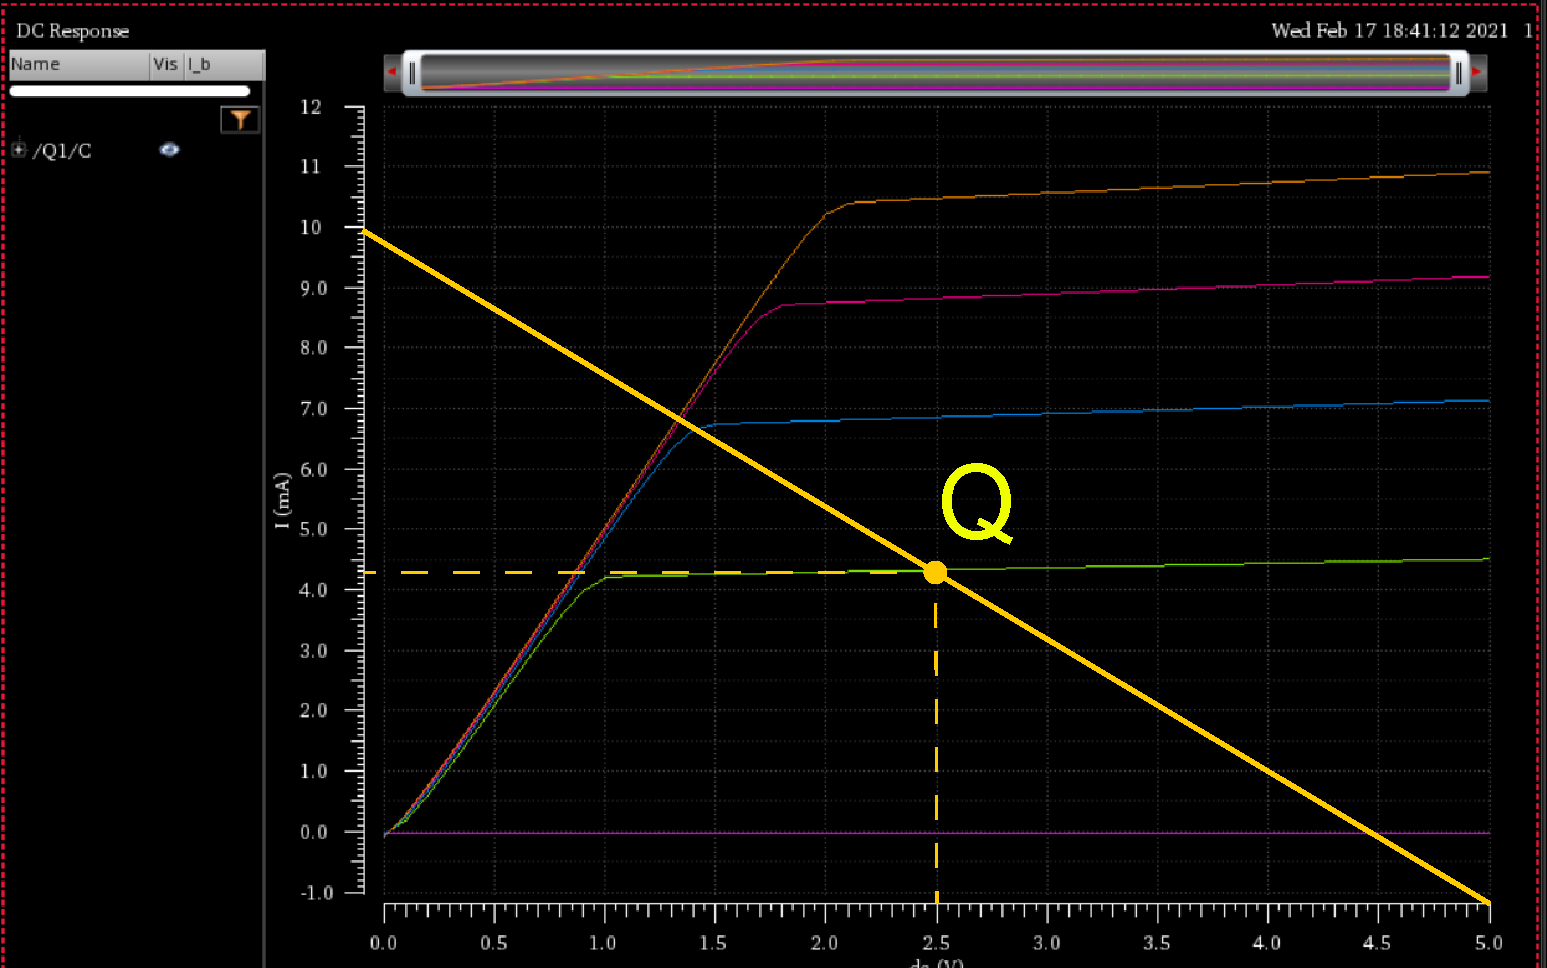
\includegraphics[width=0.2\linewidth]{1.pdf}}
\caption{План приміщення.}
\end{figure}

\end{landscape}

Висновок:  за даних умов приміщення не відповідаає нормам освітлення, тому є дисить велика потреба у штучному освітленні. Треба додати ще декілька додаткових лампочок.











\end{document}
